\documentclass[11pt]{scrartcl}
%\documentclass[11pt, twoside, a4paper, BCOR8mm, DIV12, bibtotoc,idxtotoc]{scrbook}
%\documentclass[11pt, twoside, a4paper, BCOR8mm, DIV12, bibtotoc,idxtotoc]{scrbook}
\usepackage{german}
\usepackage{path}
\usepackage{typearea}
\usepackage[utf8]{inputenc}
\usepackage{longtable}
\usepackage{hyperref}
\usepackage{graphicx}

% Zusaetzliche Picture-Umgebungen (z.B. shadowenv)
% \usepackage{picins}

% Header anpassbar
\usepackage{fancyhdr}

% Headings umdefinieren
\pagestyle{fancy}
\renewcommand{\sectionmark}[1]{\markboth{#1}{#1}}
\renewcommand{\subsectionmark}[1]{\markright{#1}}
\fancyhf{}
%\fancyhead[L]{\nouppercase{\rightmark}}
\fancyhead[L]{\nouppercase{\leftmark}}
\fancyhead[R]{\thepage}
%\fancyfoot[L]{\scriptsize O. Flimm, Anreicherungen, Mashups und
%  Vernetzungen von Titeln in einem heterogenen Katalogverbund am
%  Beispiel des Kölner UniversitätsGesamtkatalogs KUG \textbf{in:} \emph{in: Handbuch Bibliothek 2.0, Hrsg. von Julia Bergman und Patrick Danowski, Berlin, New York: De Gruyter Saur, 2010, S. 293-316. (CC-BY)}}
\parindent0.0mm
\parskip0.3cm    
\typearea{12}

\addtolength{\headheight}{8mm}
\addtolength{\headwidth}{1cm}

%\addtolength{\headheight}{7mm}
%\addtolength{\headwidth}{1cm}

\addtolength{\oddsidemargin}{11mm}
\addtolength{\evensidemargin}{-11mm}

\setkomafont{title}{\fontfamily{cmss}\fontseries{bx}\fontshape{n}\fontsize{10}{10pt}\selectfont}

\setcounter{secnumdepth}{1}

\title{Anreicherungen, Mashups und Vernetzungen von Titeln in einem heterogenen Katalogverbund am Beispiel des Kölner UniversitätsGesamtkatalogs KUG}

\author{Oliver Flimm \texttt{<flimm@ub.uni-koeln.de>}}

\date{31.3.2010}
\begin{document}

\begin{titlepage}

\maketitle

\enlargethispage{10cm} 
\thispagestyle{empty}
\begin{abstract}
\parindent0.0mm
\parskip0.3cm    
Der Kölner UniversitätsGesamtkatalog (KUG) besteht aus einer Vielzahl
einzelner Katalogbestände, darunter allein 143 separate
Institutskataloge. Aufgrund den dort vorherrschenden abweichenden
Erfassungspraktiken, z.B. in der sachlichen Erschließung, müssen
alternative Strategien angewendet werden, um für die Recherchierenden
dennoch ein Höchstmaß an Homogenität in den ansonsten heterogenen
Datenbeständen zu verwirklichen.

Diese Homogenisierung gilt sowohl für Verbesserungen der
Recherchierbarkeit von Titeln, wie auch für deren Anreicherung mit
weiteren interessanten Inhalten "= kommen sie nun aus unserem eigenen
System, von externen Diensten oder werden wiederum für externe Dienste
nutzbar gemacht. Im KUG nähern sich so klassische Kataloganreicherung
und Mashups einander an und führen im Interesse unserer Nutzer zu
einer weitgehenen Vernetzung von Titeln, zusätzlichen Inhalten und
verschiedenen Diensten.

Ermöglicht wird dies durch eine Kombination von a) Mashups mit
gängigen externen Diensten, b) einer eigenen Anreicherungsdatenbank,
in der die benötigten Vernetzungsinformationen und Inhalte für alle
Katalogbestände gesammelt werden und c) einem Eingriff in die
Synchronisation der Datenbestände des KUG mit den Erfassungssystemen,
um auch jenseits der zentralen Anreicherungsdatenbank automatisch
gezielt Inhalte in die einzelnen Kataloge einzuschleusen.

Die Anreicherungsdatenbank ist das zentrale Bindeglied zwischen den
ansonsten einzelnen Katalogbeständen im KUG. Gerade sie bietet sich
mit den dort enthaltenen Informationen als "`Andockpunkt"' für Mashups
mit dem KUG durch von ihm bereitgestellte Konnektoren an. Ein Beispiel
ist der Verfügbarkeits-Konnektor, der die Grundlage für eine
Integration der KUG-Bestände in Amazon oder Google Books bildet.

Die Heterogenität der KUG-Bestände "= ursprünglich ein Problem "= ist so
zu einer zentralen Voraussetzung geworden, um geeignete Strategien zu
entwickeln und Stukturen für eine weitgehende Vernetzbarkeit zu
schaffen. 
\end{abstract}
\end{titlepage}

\tableofcontents
\section{Motivation}

Der Katalog als Nachweisinstrument der in einer Bibliothek verfügbaren
Medien gehört zu einer der zentralen Dienstleistungen für den
Nutzer. Daher gilt es ihn zeitgemäß weiter zu entwickeln und dem
Recherchierenden bessere und vielfältigere Möglichkeiten zu eröffnen,
um an thematisch geeignete Literatur zu gelangen. Anhand des Kölner
UniversitätsGesamtkatalogs KUG werden einige der dort umgesetzten
Erweiterungen im Kontext allgemeiner Prinzipien und Techniken
erläutert, mit denen die von der Bibliothek erbrachte Dienstleistung
verbessert wurde.

\section{Die Bibliotheken der Universität zu Köln}

Die Universität zu Köln verfügt über ein sog. "`zweischichtiges
Bibliothekssystem"'\cite{Bauer:2004} in dem es neben einer zentralen
Universitätsbibliothek, der Universitäts- und Stadtbibliothek Köln
(USB Köln), eine Vielzahl an Instituts- und Seminarbibliotheken gibt.
So kommt die Universität auf insgesamt mehr als 140 verschiedene
Bibliotheken.

Im Jahr 2001 wurde das Projekt "`Kölner UniversitätsGesamtkatalog"'
begonnen, um für den Endnutzer eine "`funktionale Einschichtigkeit"'
in Form eines zentralen Bestandsnachweises aller an der Universität
elektronisch katalogisierten Medien zu erreichen. Dadurch wurden
zusätzlich weitere Synergieeffekte zwischen den Bibliotheken sowie
eine größere Homogenität in dieser hochgradig heterogenen
Bibliothekslandschaft ermöglicht.

In diesem Projekt wurden die Institutsbibliotheken unter Federführung
der USB Köln mit einem einheitlichen integrierten
Bibliothekssystem\footnote{OCLC SISIS SunRise} ausgestattet, das von
der USB betrieben und technisch über Citrix-Klienten in der
Universität bereitgestellt wird. Auf einem einzigen Serversystem in
der USB werden die einzelnen Bibliothekskataloge in separaten
Datenbanken unter einer Installation der Bibliothekssystem-Software
betrieben. Durch die Trennung können die dort verarbeiteten sensiblen
Ausleih- und Erwerbungsdaten zwischen den einzelnen Bibliotheken
bestmöglich geschützt werden.

\section{Der "`KUG"' als zentrales Nachweisinstrument}

Als zentrale Recherche-Plattform der Katalogbestände für den Endnutzer
"= Wissenschaftler, Dozenten, Studenten und Bibliothekare "= wird an
der USB Köln die Open Source Portalsoftware OpenBib\cite{Flimm:2007}
als "`Kölner UniversitätsGesamtkatalog"' oder kurz "`KUG"' eingesetzt.

OpenBib ist in seiner Architektur ein klassisches "`Schattensystem"',
in dem die Recherche von den verschiedenen Erfassungssystemen strikt
getrennt ist. Es verfügt über eine eigenständige Datenhaltung und
speichert die bibliographischen Daten eines jeden Bibliothekskatalogs
getrennt in einer eigenen relationalen Datenbank und einem eigenen
Suchmaschinenindex ab. Bei der nächtlichen Aktualisierung der
Datenbestände werden diese zunächst auf ein Zwischenformat
vereinheitlicht und dann standardisiert weiterverarbeitet. In diesen
Migrationsprozess kann eingegriffen werden, um die Daten automatisiert
zu manipulieren.

Durch die Verwendung eines Zwischenformats lassen sich Daten sehr
effizient aus beliebigen Erfassungssystemen integrieren, da lediglich
ein Konvertierungsprogramm in das Zwischenformat erstellt werden muss.
Trotz der Konsolidierung auf ein einheitliches Erfassungssystem ist
diese Fähigkeit im Institutsbereich sehr wichtig. So katalogisieren
einige unserer Institute originalsprachlich "= z.B. das Ostasiatische
Seminar mit seinen Abteilungen Japanologie und Moderne China Studien
"= und konnten daher mit ihren besonderen Schriftzeichen unsere
vereinheitlichte Bibliothekssystemsoftware aufgrund dort fehlender
UTF8-Fähigkeit bisher nicht verwenden. Der KUG unterstützt UTF8 und
kann daher auch diese Kataloge problemlos wie all die anderen
integrieren und so einen tatsächlichen Gesamtnachweis aller
elektronisch erfassenden Institutsbibliotheken bereitstellen. Auch
jenseits der Bibliotheksbestände werden in den KUG viele weitere
relevante Datensammlungen integriert, wie z.B. der
Hochschulschriftenserver der Universität, Research Papers in
Economics, Digitalisate der Open Library uvm.

Der KUG stellt den Nutzern eine zeitgemäße moderne
Rercherche-Technologie mit facettierter Suche und vielen weiteren
Funktionen bereit. Mit Tagging und Literaturlisten werden die Anwender
konsequent bei der Erstellung von Inhalten in die KUG-Plattform
einbezogen und können so einen Mehrwert für alle anderen Anwender
liefern. Bereits die einfache Nutzung des KUG genügt, um später durch
geeignete Analysen des Anwenderverhaltens neue Inhalte zu erzeugen.

Eine der Grundstrategien im KUG ist die maximal mögliche thematische
Vernetzung der Katalogdaten, sowohl innerhalb eines einzelnen, wie
auch aller Kataloge - und zusätzlich mit weiteren externen
Informationen. Dazu versuchen wir aktiv die Auffindbarkeit von Titeln
durch den Nutzer zu verbessern. Durch den Einsatz eines
Templating-Systems wird die Präsentation von Inhalten gesteuert und
ist so sehr flexibel einsetzbar über verschiedene Abstraktionsebenen
hinweg - Kataloge, Gruppen von Katalogen und die finale Präsentation
in Sichten auf eben jene Kataloggruppen.

Aufgrund der Ausgangssituation mit vielen heterogenen Datenbeständen
und der z.T. uneinheitlichen Erfassung in Bezug auf Verschlagwortung,
Systematisierung oder die Vergabe von Medientypen, müssen für eine
Vereinheitlichung und Anreicherung andere Wege beschritten werden, als
bei einem einzelnen Katalog "`im Vakuum"'.  Ebensowenig existiert das
KUG-Gesamtsystem mit seinen vielen Datenbanken in einem Vakuum,
sondern muss durch offene Schnittstellen für seine Dienste und Daten
in das es umgebende Netz eingebettet werden.

\section{Automatisierte und zentrale Kataloganreicherung}

"`Mit Kataloganreicherung (englisch catalog enrichment) werden
Einträge eines Bibliothekskatalogs um weiterführende Informationen
ergänzt, die über die reguläre Formal- und Sacherschließung
hinausgehen."'\footnote{Wikipedia:
  \path|http://de.wikipedia.org/wiki/Kataloganreicherung|. Zuletzt
  besucht am: 26.3.2010}. Im Kontext der besonderen Situation eines
Verbundes einzelner Erfassungssysteme werden insgesamt zwei Arten von
Kataloganreicherungen im KUG verwirklicht.

Da ist zunächst eine automatisierte Anreicherung, die in den
Prozess des Einspielens eines Katalogs in den KUG integriert ist.
Durch diese Anreicherung werden die Daten für die Recherche durch den
Nutzer verbessert.

Ein Problem ist hier beispielsweise die unvollständige Kennzeichnung
der Titel mit rudimentären Medientypen wie Zeitschrift oder Aufsatz.
Daher wird beim Neuaufbau eines Kataloges im KUG jeder Datensatz
kategorieweise analysiert und anhand verschiedener Kriterien eben jene
Medientypen bestimmt und hinzugefügt.

Ein anderes Problem liegt in besonderen Erfassungsspezifika und dem
Umstand, dass ein gewöhnliches Recherchesystem einen Titelsatz
lediglich anhand der in ihm vorkommenden Informationen finden kann. Im
Schiller-Räuber-Problem ist dies aber nicht der Fall, da beide
Informationen in verschiedene Titelsätze disjunkt verteilt sind
"= typischerweise "`Schiller"' in der Hauptaufnahme "`Werke"' und "`Die
Räuber"' in der untergeordneten Aufnahme ohne Nennung der Person
"`Schiller"'. Daher muss in der untergeordneten Titelaufnahme auch die
Person der übergeordneten Aufnahme für die Recherche herangezogen
und indexiert werden.

Als letztes Beispiel sei die Problematik ISBN10/13 genannt, bei der
Titel ehemals mit einer ISBN10 aufgenommen wurden, diese nun aber mit
der zugehörigen ISBN13 recherchiert werden. Auch hier ist der
Suchindex geeignet zu modifizieren, so dass unabhängig von der
ISBN-Variante der jeweilige Titel gefunden werden kann.

Bei der Anreicherung der Titel mit externen Inhalten bestehen in einem
Katalogverbund wie dem KUG, mit vielen getrennten Katalogen,
erschwerte Bedingungen. Einerseits ist der Aufwand, diese
Informationen in die vielen "= teils verschiedenen "= primären
Erfassungssysteme einzuladen und aktuell zu halten, sehr hoch.
Andererseits lehnen einige Bibliothekare die "`Verunreinigung"' der
von ihnen erfassten Katalogdaten tendenziell eher ab.

Daher haben wir diese Art der Anreicherung direkt in das KUG
Rercherchesystem in Form einer separaten zentralen
Anreicherungsdatenbank integriert. In dieser werden verschiedene
Informationen zur Nutzung durch alle Kataloge abgelegt. Als
Identifizierungsschlüssel dienen ISBN, ISSN bzw. der
Bibkey\footnote{\path|http://www.gbv.de/wikis/cls/Bibliographic\_Hash\_Key|.
  Zuletzt besucht am: 26.3.2010} "= ein "`bibliographischer
Fingerabdruck"' des entsprechenden Titels.

Zu den zentral gesammelten Inhalten gehören zunächst einmal
kategoriebasierte Inhalte. Die anzureichernden Informationen werden
dazu unter einer numerischen Kategorie in der Datenbank abgelegt.
Zusätzlich wird die Herkunft der Anreicherung kodiert hinzugefügt.
Damit lassen sich gleichartige Inhalte aus verschiedenen Quellen
nachträglich auseinander halten und besser aktualisieren. Ein Beispiel
sind URL's auf universitätsweit lizensierte E-Books, die mit ihrer
Print-ISBN13 dort in der Kategorie 4120 abgelegt werden.

Weiterhin wird zentral ein katalogübergreifender Gesamtnachweis aller
Titel aus allen getrennten Katalogen aufgebaut. Um auf einen Blick die
Existenz des Titels und die Zugehörigkeit zu einem bestimmten Katalog
festzustellen und somit eine Anreicherung auch wieder in den Kontext
des lokalen Katalogbestandes zu rücken, werden sowohl die
Identifikationsnummer als auch der Katalogname eines jeden Titels
unter der ISBN, ISSN bzw. dem Bibkey in der Datenbank abgelegt.

Zusätzlich sind dort die Gesamtnachweise aller ISBN’s zu einem Werk
angesiedelt: Alle ISBN’s eines Werkes, also derselbe Titel in
verschiedenen Ausgaben, Sprachen usw., werden in der Datenbank
abgelegt. Als Datenlieferanten nutzt der KUG LibraryThing und die
ThingISBN\footnote{\path|http://www.librarything.com/thingology/2006/06/introducing-thingisbn\_14.php|.
  Zuletzt besucht am: 26.3.2010}.

Schließlich wird dort auch noch ein katalogübergreifender
Gesamtnachweis der Ansetzungsformen von Normdaten geführt, um dem
Nutzer z.B. effizient Suchvorschläge für seine Recherche aufgrund des
tatsächlichen Bestands anbieten oder einen effizienten
katalogübergreifenden Normdaten-Index verwirklichen zu können.

Der Vorteil dieser zentralen Anreicherungsdatenbank ist, dass die
Anreicherungsinformationen nun nicht mehr mit einem speziellen Titel
in einem speziellen Katalog verknüpft sind, sondern stattdessen von
diesen getrennt "= "'freischwebend"' "= gehalten werden und dadurch
automatisch nutzbar für alle Kataloge über die ISBN, ISSN bzw. den
Bibkey sind. Der jeweilige Titel in irgendeinem Katalog "`weiß"'
selbst nichts von einer möglichen Anreicherung seiner
bibliographischen Daten.

Erst bei der Einzeltrefferanzeige werden für einen konkreten Titel
Katalog- und Anreicherungsdaten kombiniert und dann ausgegeben. In
diesem Sinne stellt die im KUG verwendete zentrale Kataloganreicherung
eine Form eines "`internen Mashups"' dar.

Für eine effiziente Anreicherung bei der Recherche können gezielt
beliebige Anreicherungsinhalte in den Suchindex eines Kataloges
übernommen werden. Ein gutes Beispiel hierfür ist die Anreicherung
eines Titels mit den Namen der Artikel, die ihn in der Wikipedia
zitieren. Auf diese Weise werden dem Titel weitere Informationen für
die Recherche hinzugefügt und er kann vom Endnutzer besser gefunden
werden. Der Titel "`Vergleichende Primatologie"' von Thomas Geissmann
wird so z.B. für die Recherche um unzählige Namen von Affenarten
erweitert.

\subsection{Beispiel: Kataloganreicherung mit Schlagworten}

In den verschiedenen Katalogen des KUG trifft der Endnutzer auf eine
höchst unterschiedliche sachliche Erschließung. Für den gleichen Titel
werden entsprechend dem verwendeten Regelwerk "= die USB
verschlagwortet nach RSWK "= oder den Vorlieben der jeweiligen
InstitutsbibliothekarInnen "= dort wird frei, aber oft näher am
Fachgebiet verschlagwortet "= verschiedene Schlagworte vergeben. Dazu
kommt, dass im besten Fall immerhin noch verschiedene, im schlimmsten
Fall jedoch gar keine Schlagworte vergeben werden. Einmal abgesehen
von der verwirrenden und uneinheitlichen Erscheinungsform des Titels
in der Vollanzeige für den Recherchierenden, kann dieser den Titel in
einem Katalog eventuell über die Suche nach dem entsprechenden
Schlagwort finden, im anderen aber gerade nicht.

Dieses Problem lässt sich sehr einfach mit der zentralen
Kataloganreicherung im KUG lösen.

Dazu werden in einem ersten Schritt bei der nächtlichen Aktualisierung
eines jeden Katalogs im KUG die dort vergebenen Schlagworte mit der
zugehörigen ISBN als Zugriffsschlüssel in unserer zentralen
Anreicherungsdatenbank abgelegt. Damit wurden bereits folgende zwei
Ziele erreicht. Zunächst stehen nun jeder Titelaufnahme über ihre ISBN
alle korrespondierenden "`angereicherten"' Schlagworte jenseits der
(etwaig vorhandenen) lokalen Verschlagwortung zur Verfügung.
Zusätzlich wird durch die Anreicherungdatenbank ein Verknüpfungsnetz
von Titeln, identifiziert durch alle ISBNs zum jeweiligen Schlagwort
"= quasi unsichtbar "= über den aktuellen (Teil-)Katalog gelegt. Auf
diese Weise lassen sich zu jedem so angereicherten Schlagwort auch
weitere thematisch gleich eingeordnete Titel im aktuellen Katalog
finden und verknüpfen "= auf Grundlage der Verschlagwortung des Titels
in einem anderen Katalog.

Im KUG werden diese "`angereicherten Schlagworte"' mit entsprechender
Verknüpfung in der Einzeltrefferanzeige im Block "'Entdecken Sie
weitere Treffer über:"' als "`Verschlagwortung aus anderen Katalogen"'
angezeigt "= für den Recherchierenden bewusst getrennt von den
sonstigen bibliographischen Daten.

In einem zweiten Schritt werden nun nur noch durch entsprechende
Parametrisierung die "`angereicherten Schlagworte"' mit in den
Suchindex des jeweiligen Katalogs übernommen und sind so neben den
"`normalen"' Schlagworten recherchierbar. Ein derart mit weiteren
Schlagworten angereicherter Titel profitiert unmittelbar von dieser
Anreicherung, weil die Wahrscheinlichkeit steigt, dass er "`mit den
Suchworten des Recherchierenden"' auch gefunden wird. Die Grundannahme
ist also: Je größer die Wortbasis der intellektuell verschlagwortenden
BibliothekarInnen, desto größer auch die Wahrscheinlichkeit, dass der
Nutzer mit einem davon recherchiert und dadurch den Titel findet.

Ein gutes Beispiel für diese Kataloganreicherung mit Schlagworten ist
der Titel "`Die materielle Polizeipflicht des Zustandsstörers und die
Kostentragungspflicht nach unmittelbarer Ausführung und Ersatzvornahme
"= dargestellt am Beispiel der
Altlasten-Problematik"'\footnote{PermaLink:
  \path|http://kug.ub.uni-koeln.de/portal/connector/permalink/inst201/44212/1/kug/index.html|.
  Zuletzt besucht am: 26.3.2010} von Michael Griesbeck aus dem Katalog
der Fachbibliothek Rechtswissenschaft (Abbildung \ref{bild:verschlagwortung}).

Dieser Titel wurde lokal mit den Worten Altlasten, Kostenpflicht und
Polizeipflicht verschlagwortet. Durch die Anreicherung kommen nun noch
die Begriffe Altlastsanierung, Störer, Zustandshaftung und
Gefahrenabwehr hinzu.

%\begin{shadowenv}
\begin{figure}
    \centering \begin{minipage}[b]{1.0\textwidth}
      \centering 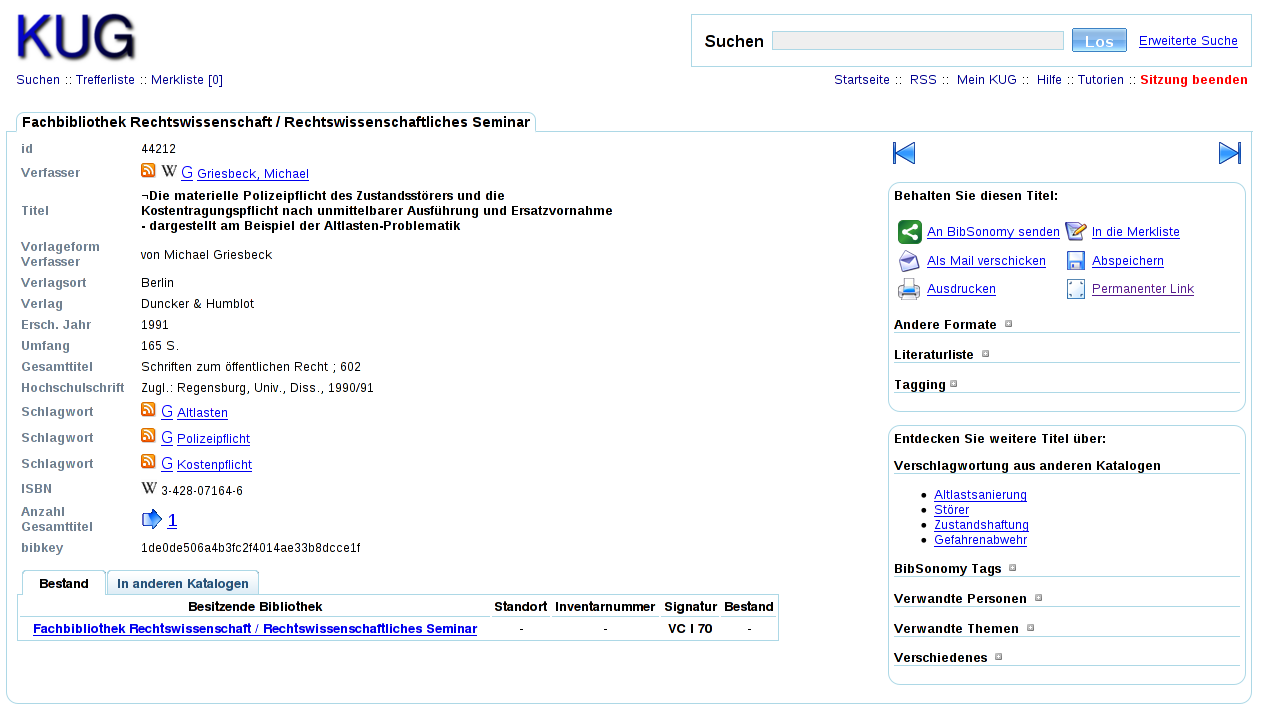
\includegraphics[width=15cm]{bib20-kug-mashups_bilder/swtenrich1.png}
    \end{minipage}
    \caption{Beispiel für die Integration der Verschlagwortung in anderen Katalogen}
  \label{bild:verschlagwortung}
\end{figure}
%\end{shadowenv}


Gleichzeitig ist dieser Titel auch im Katalog des Instituts für
Öffentliches Recht und Verwaltungslehre vorhanden.
 
Dort ist der Titel überhaupt nicht verschlagwortet und er profitiert
maximal von der Anreicherung. Mehr noch "= wie bereits angesprochen
können alle Titel durch den Nutzer in diesem Katalog erreicht werden,
die auch in anderen Katalogen vorhanden sind und dort entsprechend
verschlagwortet wurden "= z.B. mit dem Schlagwort Gefahrenabwehr
ergeben sich so 5 zusätzlich vernetzte Titel.

Die Kataloganreicherung mit Schlagworten ist ein gutes Beispiel dafür,
wie mit relativ wenig Aufwand für den Recherchierenden ein deutlicher
Mehrwert im Bereich Recherchierbarkeit sowie thematische
Titelvernetzung geschaffen werden konnte.

Zusätzlich zu den intellektuell erfassten bibliographischen Daten und
ihrer Erschließung kann sich die Auffindbarkeit von Titeln durch die
automatische Verarbeitung verschiedener titelbezogener Informationen
wie Inhaltsverzeichnisse, Register und Glossare anhand linguistischer
sowie semantischer Methoden weiter verbessern lassen. Eine Erweiterung
des KUG um solche Techniken steht zur Zeit noch aus.

Der Einsatz der Kataloganreicherung "= automatisch und zentral "=
stellt ein wesentliches Werkzeug in einem Verbund unabhängiger
Kataloge dar, um für den Nutzer "= neben dem Zugewinn an
Auffindbarkeit und Information "= eine Homogenität zwischen den
Katalogen zu schaffen, die ursprünglich gar nicht existierte.

\section{Vernetzung durch Mashups}

Unter einem Mashup versteht man die "`Erstellung neuer Medieninhalte
durch die nahtlose (Re-)Kombination bereits bestehender
Inhalte"'\footnote{Wikipedia:
  \path|http://de.wikipedia.org/wiki/Mashup\_(Internet)|. Zuletzt
  besucht am: 26.3.2010} . Im Web 2.0 gehören sie zu einer häufig
genutzten Technik, um externe Dienste mit ihren Inhalten in die eigene
Anwendung unter Verwendung von Zugriffsschnittstellen (API's)
einzubinden. Der externe Dienst wird über das Internet direkt
angesprochen und liefert seine Informationen zurück.

Häufig geschieht dies durch den Einsatz von JavaScript und AJAX direkt
auf einer Webseite und damit effektiv im Browser des Endnutzers. Die
Verknüpfung und Verarbeitung externer Informationen kann aber auch in
die jeweilige Anwendung integriert sein. Dann kommuniziert die eigene
Anwendung mit dem Dienst und verarbeitet die Informationen danach
selbst intern weiter.

Die Nutzung eines externen Dienstes über einen Mashup stellt einen
sehr effizienten Mechanismus dar, da der Aufwand entfällt, diesen
Dienst selbst lokal zu implementieren und somit das Rad neu zu
erfinden.

Einer der bekanntesten und am häufigsten genutzten Dienste ist Google
Maps für die Integration geographischen Kartenmaterials. Andere
Beispiele sind Flickr, YouTube oder SlideShare.

Auch im Kontext von Bibliothekskatalogen kann die Technik von Mashups
sinnvoll angewendet und so ein Mehrwert für den Endnutzer erreicht
werden\cite{Hahn:2009}\cite{Stelzenmueller:2008}.
	
Ebenso wie bei der automatischen und zentralen Kataloganreicherung im
KUG können Mash\-ups direkt für alle Kataloge eingesetzt werden und sind
daher gerade in unserem Verbund separater Kataloge ein sehr geeignetes
Werkzeug einen Mehrwert bei gleichzeitig geringem Arbeitsaufwand zu
liefern. Dazu reicht es i.A. aus, ein entsprechendes
JavaScript-Fragment in einem geeigneten katalogübergreifend genutzten
Ausgabe-Template abzulegen.

Als Alternative für den Einsatz von JavaScript werden einige Inhalte
auch über einen eigenen KUG-Dienst AvailabilityImage ausgegeben, der
Verfügbarkeiten in externen Systemen über ein Bild signalisiert.

Dieses "`Bild"' wird über einen URL verlinkt, der die Recherche bzw.
den Einsprung in den jeweiligen externen Dienst aufruft "=
üblicherweise mit der in der Titelaufnahme enthaltenen ISBN. Das
"`Verfügbarkeits-Bild"' wird dann dynamisch über den lokalen
AvailabilityImage-Dienst erzeugt.

Dieser überprüft "= ebenfalls über eine einfache Recherche "= die
Verfügbarkeit von Informationen über den aktuellen Titel im entfernten
System. Existieren Informationen zum aktuellen Titel, so wird ein
geeignetes Status-Bild per internem Redirect ausgegeben und der
Recherche-Link ist nutzbar.  Im anderen Fall wird stattdessen ein
transparenter Pixel ausgegeben und der Link ist unsichtbar. Dieses
sehr einfache Verfahren hat sich insbesondere in den Fällen bewährt,
wenn gerade (noch) kein API vorhanden ist, wie es z.B. bis März 2010
beim "`Internet-Copy-Shop"' PaperC der Fall war. Insgesamt hat sich
jedoch der Einsatz von API's durchgesetzt.

\begin{figure}
    \centering \begin{minipage}[b]{1.0\textwidth}
      \centering 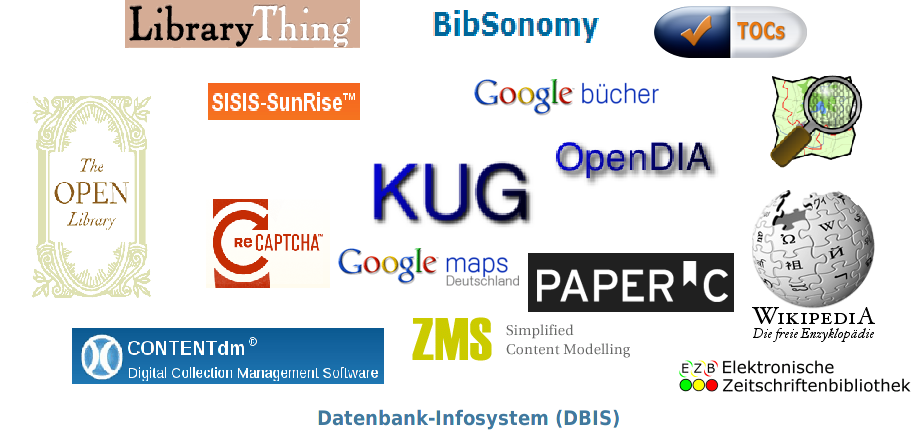
\includegraphics[width=15cm]{bib20-kug-mashups_bilder/mashups.png}
    \end{minipage}
    \caption{Konsequente Nutzung externer Dienste im KUG}
  \label{bild:mashups}
\end{figure}

Weit verbreitet bei API's sind hier Umsetzungen mit REST
(Representational State Transfer), XML-RPC und SOAP sowie JSON bzw.
XML als Format für die Antwort auf eine Anfrage.

Im KUG versuchen wir die Möglichkeiten, die das Netz mit seinen
Diensten bietet, konsequent zu nutzen (Abbildung \ref{bild:mashups}).

Google Bücher liefert weitergehende Informationen wie ausführliche
Inhaltsbeschreibungen und Inhaltsverzeichnisse, Verweise auf das
aktuelle Buch in anderen Büchern oder Artikeln usw.

Google Maps liefert Kartenmaterial, so dass im Kontext allgemeiner
Informationen zu einer Bibliothek "= wie sie an der USB im sog.
Bibliotheksführer für alle Bibliotheken an der Universität zu Köln
erfasst werden "= innerhalb des KUG auch die Position der jeweiligen
Bibliothek auf einem Kartenausschnitt verzeichnet werden kann.

Open Library liefert in Kombination mit Google Bücher für den KUG
Bilder von Buch-Covern. TicTocs/JOURNAL TOCs liefert eine Übersicht
der zuletzt in einer Zeitschrift veröffentlichten Artikel, teilweise
mit Inhaltszusammenfassung und direkter Verlinkung des Artikels.

ReCaptcha schützt die freie Registrierung von Endnutzern für den KUG
vor automatisiertem Zugriff und dem damit verbundenen
Missbrauchspotential. Über PaperC können Bücher kostenfrei online
gelesen werden.

Und schließlich werden die Elektronische Zeitschriftenbibliothek EZB
und das Datenbankinformationssystem DBIS über thematisches Browsing
und die gezielte Suche nach Zeitschriften sowie Datenbanken
eingebunden.

\subsection{Beispiel: Integration von BibSonomy}

Aufgrund seiner konzeptionellen Bedeutung, die deutlich über die
bisher genannten Mashups hinaus geht und als Beispiel für einen direkt
in die KUG-Plattform integrierten Dienst wird nun auf das "`Social
bookmark and publication sharing system"`
BibSonomy\footnote{\path|http://www.bibsonomy.org/|. Zuletzt besucht
  am: 26.3.2010} näher eingegangen.

Bereits Anfang 2007 wurde der KUG um eine eigene Tagging-Funktion
erweitert. War diese zunächst noch eine zeitgemäße Alternative zu
klassischen strukturierten Merklisten, wurde wenig später durch die
Öffnung öffentlich markierter Tags für andere auch eine
gemeinschaftliche Nutzung ermöglicht. Dieses
Social-Tagging\cite{Voss:2007}\cite{Tonkin:2008} auf lokaler Ebene
bringt jedoch auch Probleme mit sich.

Das größte Problem besteht in der lokal nicht erreichten kritischen
Masse und Zersplitterung der Nutzer. Die potentielle Nutzerschaft für
einen lokalen Katalog ist typischerweise begrenzt. Für ein
erfolgreiches Social-Tagging ist aber eine kritische Masse an
Endanwendern notwendig, die entsprechend aktiv ist. Durch die Existenz
diverser Bibliothekskataloge - eine Universität, eine Bibliothek, ein
Katalog - findet aber zwangsläufig eine Zersplitterung statt. Der
mögliche erreichbare Nutzen ist nicht optimal.

Darüber hinaus werden die lokal vergebenen Tags ein Datensilo im
Rechercheportal. Zwar sind die Katalogdaten durch vielfältige
Exportmöglichkeiten ‘befreit‘, die lokal vergebenen Tags sind aber in
der Rechercheanwendung eingeschlossen und bilden so ein eigenes
Datensilo. Auch diesen Umstand gilt es zu verbessern.

Vor diesem Hintergrund ist es sehr ratsam, die lokale
Rechercheplattform mit anderen Systemen zu kombinieren, die dann als
Datenaggregator auftreten und über eine entsprechend hohe Nutzerzahl
verfügen, mit der sie die so wichtige kritische Masse erreichen.

Typische Beispiele für solche Dienste sind BibSonomy und Connotea und
auch das ursprünglich nur lokal nutzbare Zotero beschreitet den
Weg zu einer vielversprechenden kollaborativen Plattform.

Für den KUG fiel die Wahl auf BibSonomy. Dieses System verfügt über
ein eigenes API und kann daher ideal als Mashup in den KUG eingebunden
werden.

Neben der - schon vor dem Einsatz des BibSonomy-API existierenden -
Möglichkeit im KUG einzelne Titel gezielt nach BibSonomy zu
übertragen, können nun "= mit dem API"= alle bibliographischen
Nachweise und Web-Quellen in BibSonomy vollständig mit einem
thematischen Browsing über Tags und Schlagworte erschlossen werden.
Darüber hinaus findet eine "`Spiegelung der lokalen Tagging-Aktionen"'
in BibSonomy statt.

Hintergrund des "`thematischen Browsens"' ist der Wunsch, über die
zentrale Datenbasis von BibSonomy anhand von Tags oder Schlagworten
weitere thematisch infrage kommende Quellen "= Publikationen und
Bookmarks "= zu entdecken. Damit wird dem Aspekt Serendipity "`Ich
möchte auch etwas finden, was ich gar nicht gesucht
habe"'\footnote{Beluga Blog:
  \path|http://beluga-blog.sub.uni-hamburg.de/blog/2008/02/22/wenn-das-klima-anders-waere\newline-koennte-man-auch-eine-unfertige-liste-oeffnen-beluga-in-der-diskussion/|.
  Zuletzt besucht am: 26.3.2010} Rechnung getragen.

Dazu wird zunächst bei der Einzeltrefferanzeige eines Titels im KUG
mit dem Bibkey (konkreter: dem derzeitigen inter-hash
key\footnote{\path|http://www.bibsonomy.org/help/doc/inside.html|.
  Zuletzt besucht am: 26.3.2010} von BibSonomy) eine Abfrage in
BibSonomy gemacht und der aktuelle Titel gesucht. Alle Tags, die
gegebenenfalls beim dort gefundenen Titel vergebenen wurden, können
dann anschließend im KUG unter dem Abschnitt "`BibSonomy Tags"'
ausgegeben werden.

Da nicht jeder Titel aus dem KUG schon in BibSonomy vorhanden ist,
werden zusätzlich die im KUG-Titel verwendeten Schlagworte "`als
Tags"' mit BibSonomy abgeglichen (Abbildung \ref{bild:bibsonomy}).

\begin{figure}
    \centering \begin{minipage}[b]{1.0\textwidth}
      \centering 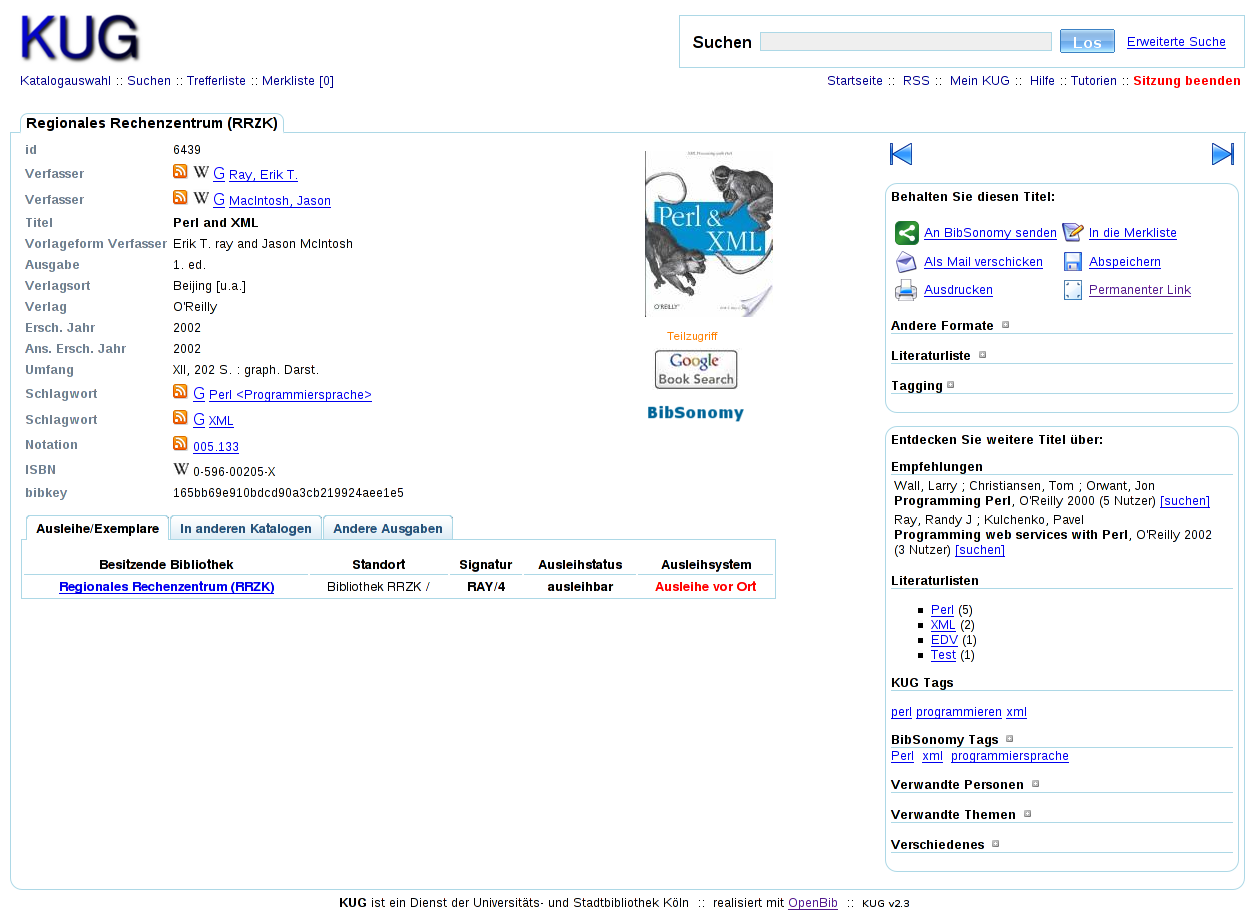
\includegraphics[width=15cm]{bib20-kug-mashups_bilder/bibsonomytitel.png}
    \end{minipage}
    \caption{Beispiel für die Verbindung eines Titels zu BibSonomy anhand von Tags und Schlagworten}
  \label{bild:bibsonomy}
\end{figure}

Auf diese Weise erhält der Nutzer schließlich eine Aufstellung valider
Tags, über die er in den Bestand von BibSonomy eintauchen kann und
eine Aufstellung dort vorhandener Publikationen bekommt (Abbildung
\ref{bild:bibsonomy-publist}).  Dieser automatische Abgleich mit BibSonomy ist
vollständig in die KUG-Oberfläche eingebettet.

Anhand der Bibkeys für die in BibSonomy gefundenen Publikationen wird
dann augenblicklich wieder eine Verfügbarkeitsabfrage im KUG-Bestand
gemacht, so dass für die durch BibSonomy gelieferten Titel sofort
angezeigt werden kann, ob sie im KUG-Bestand vorhanden sind. Grundlage
hierfür ist die vorherige Anreicherung der KUG-Titel mit Bibkeys sowie
der Gesamtnachweis in der zentralen Anreicherungsdatenbank.

\begin{figure}
    \centering \begin{minipage}[b]{1.0\textwidth}
      \centering 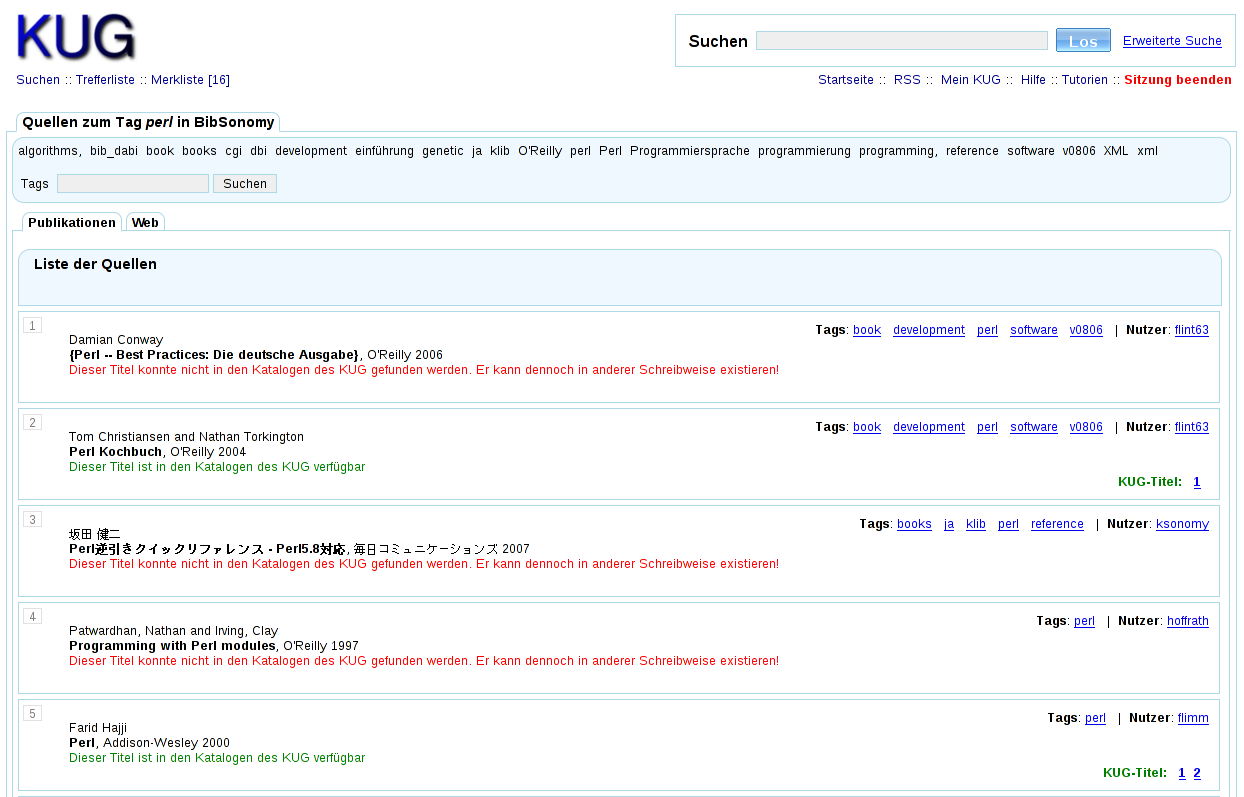
\includegraphics[width=15cm]{bib20-kug-mashups_bilder/bibsonomy-publist.png}
    \end{minipage}
    \caption{Titel zum Tag "`perl"' in BibSonomy mit weiterer Vernetzung von Tags und Nutzern}
  \label{bild:bibsonomy-publist}
\end{figure}

Stellt das "`thematische Browsing"' einen Weg dar, BibSonomy in den
eigenen Katalog zu integrieren und als die angesprochene
"`gemeinsame"' Datenbasis lokal zu nutzen, wird mit der
vollautomatischen Spiegelung der lokalen Tagging-Aktionen nach
BibSonomy genau die dazu notwendige Öffnung des Datensilos OPAC und
ein verbesserter (Katalog- und Tagging-) Datenfluss nach BibSonomy
forciert.

Dazu taggt der Endnutzer direkt im KUG. Seine Tags und Titel werden
durch den BibSonomy-Mashup nun aber nicht mehr nur im KUG gespeichert.
Darüber hinaus werden die Titel im KUG "= so sie im BibSonomy-Account
des Nutzers noch nicht vorhanden sind "= automatisch dort eingetragen
und mit den lokal im KUG vergebenen Tags und der
Sichtbarkeitsinformation (öffentlich oder privat) versehen. Ändert er
seine Tags im KUG, so werden diese Änderungen auch in BibSonomy
automatisch nachgezogen.

Auf diese Weise können die Nutzer weiterhin lokal das Rechercheportal
mit all seinen Funktionen nutzen, die Daten wandern aber zusätzlich
zur gemeinsamen ‘Datenzentrale‘ BibSonomy. Jenseits der weitergehenden
Funktionen von BibSonomy für den Nutzer, erhält er zusätzlich "=
rückgekoppelt im lokalen Kontext "= weitere Verweise auf  Literatur,
die an der Universität vorhanden ist.

\section{Mashups durch externe Datenlieferungen}

Bisher wurden Mashups vorgestellt, die sich sofort über das Netz mit
einem externen Dienst verbinden, dort Informationen sammeln und mit
der lokalen Anwendung zu etwas Neuem kombinieren. Einige Dienste
bieten jedoch auch die Möglichkeit an, die Gesamtheit der
Informationen direkt herunterzuladen. Die lokale Abspeicherung und
Verarbeitung dieser Informationen bietet dann u.a. zusätzlich die
Möglichkeit, diese Informationen auch für alle lokal vorhandenen Titel
in Nutzerrecherchen zu verwenden.

Die Verarbeitung solcher externer Daten findet im KUG zentral in der
Anreicherungsdatenbank statt. Typische Beispiele wurden bereits im
entsprechenden Abschnitt über die zentrale Kataloganreicherung
genannt. Es sind LibraryThing mit der ThingISBN für die
Gesamtnachweise aller ISBN’s zu einem Werk sowie die Wikipedia für die
Namen der Artikel, in denen auf Titel mit deren ISBN verwiesen wird.

\section{Bereitstellung eigener Dienste und Daten}

Ebensowenig wie ein einzelner Katalog im Vakuum ohne die anderen
Kataloge im KUG gesehen werden kann und man daher katalogübergreifend
denken muss, steht auch der KUG nicht für sich allein, sondern ist in
eine Welt aus Diensten und Daten eingebettet. Dementsprechend kommt
zum "`katalogübergreifenden Denken"' ein "`systemübergreifendes
Denken"' hinzu.

So hat sich der KUG über die Jahre von einer reinen 1-dimensionalen
Recherchelösung im klassischen OPAC-Sinn hin zu einem Portal-Baukasten
und einer allgemeinen Infrastrukturlösung an der USB Köln entwickelt,
die sowohl Dienste wie auch Daten zur externen Verwendung bereit
stellt. Der KUG ist nicht mehr nur ein Katalog, sondern eine
vielfältig nutzbare Plattform.

Dazu tragen speziell die verschiedenen Organisationsmöglichkeiten für
einzelne Kataloge in der KUG-Plattform bei. In nur einer Installation
des KUG lassen sich aus der Gesamtmenge aller Kataloge beliebige
Gruppen in eigenen Katalog-Profilen zusammenfassen. Diese Profile
lassen sich dann wiederum über sog. Sichten in verschiedenen
Präsentationen für den Endnutzer aufbereiten und bilden dann ein
eigenständig ansprechbares Portal.

Diese drei verschiedenen Abstraktionsebenen im KUG "= Datenbanken,
Sichten und Profile (zur Gruppierung von Datenbanken/Sichten) "=
können bequem über ein Web-Frontend verwaltet werden und übertragen
sich exakt auf das für die Web-Präsentation eingesetzte
objektorientierte Templatingsystem.

An der USB Köln können durch die so erreichte Flexibilität ohne viel
Aufwand "= jenseits der Standard-KUG-Sicht mit fast allen verfügbaren
Katalogen "= getrennte Varianten für jedes Institut sowie
eigenständige Projekt- und Themenportale eingerichtet werden. Im März
2010 summierte sich die Gesamtzahl der von der KUG-Plattform
bereitgestellten individuellen Portal-Sichten auf 183.

\begin{figure}[ht]
    \centering \begin{minipage}[b]{1.0\textwidth}
      \centering 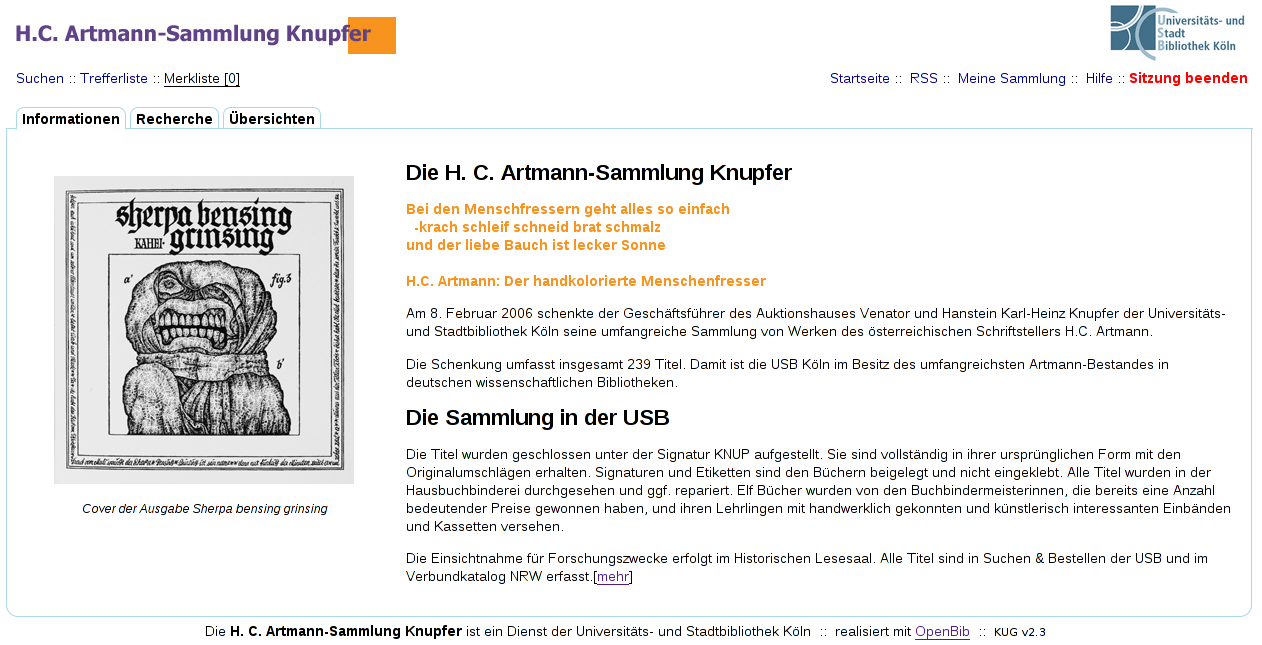
\includegraphics[width=15cm]{bib20-kug-mashups_bilder/artmann.png}
    \end{minipage}
    \caption{Die H. C. Artmann-Sammlung Knupfer als Beispiel für ein eigenständiges Portal in der KUG-Plattform}
  \label{bild:artmann}
\end{figure}

Ein gutes Beispiel hierfür sind die vielen Sammlungen der
Universitäts- und Stadtbibliothek Köln, die jedoch im Gesamtbestand
aller Titel im Katalog der USB leider weitgehend untergehen "= vielen
Nutzern erschließt sich nicht, welche Sammlungen die USB überhaupt
besitzt.

Aus diesem Grund hat die USB begonnen, Kriterien für deren
Identifikation zu bestimmen, um dann in einem ersten Schritt die
jeweilige Sammlung aus dem Gesamtbestand zu extrahieren und in eine
eigene Datenbank in der KUG-Plattform einzuspielen. Die
Sammlungsbestände werden so "= jeder für sich "= aus der Anonymität
des gesamten Kataloges herausgelöst und getrennt ansprechbar.

Dazu nutzen wir einfache Konvertierungs-Plugins, die für die Bildung
der jeweiligen Teilbestände aus dem USB Katalog sorgen. Sehr
vorteilhaft ist hier wieder die eigenständige Datenhaltung in einer
relationalen Datenbank und einem Suchmaschinenindex in der
KUG-Plattform, mit der Sammlungen auch aus verschiedenen
Erfassungssystemen dort zusammengeführt werden können. Das ist umso
wichtiger, da etliche Sammlungen an der Universität zu Köln gerade
nicht im USB-Katalog nachgewiesen sind, wir aber eine Gesamtlösung für
die Universität anstreben. Das Spektrum der vorhandenen Daten reicht
hier von der einfachen Excel-Datei bis zum spezialisierten
Erfassungsystem.

Für jede dieser Sammlungen wird eine eigene Portal-Sicht erstellt, in
der die Bestände beschrieben und über Recherchemöglichkeiten,
Übersichten und/oder Register für die Nutzer zugänglich gemacht
werden. Mit dieser individuellen Präsentation möchten wir unserer
Wertschätzung einer jeden Sammlung und eines jeden Sammlers Ausdruck
verleihen und unsere Nutzer auf diese verborgenen Schätze aufmerksam
machen (Abbildung \ref{bild:artmann}).

Neben der Fähigkeit getrennte Portale einzurichten stellt die
KUG-Plattform viele ihrer Funktionen auch durch eigene offene
Schnittstellen "= den sog. Konnektoren "= für eine externe Nutzung
bereit. Dies geschieht im Allgemeinen in Form von Web Services. Damit
lassen sich Konnektoren ideal zum Aufbau serviceorientierter
Infrastrukturen auf Basis des KUG nutzen.

Über den DigiBib-Konnektor, dessen Abfrageprotokoll auf Vorgaben des
Hochschulbibliothekszentrums NRW (hbz) beruht, können verschiedene
Kataloge sowohl in unser lokales USB-Portal wie auch mit dem
Literaturverwaltungsprogramm Citavi durchsucht werden. Hier wurde vom
hbz bewusst einem einfachen HTML-basierten Abfrageprotokoll gegenüber
dem komplexeren Standard Z39.50 der Vorzug gegeben, das einfach
implementier- und erweiterbar ist "= z.B. um Facetten bei der
Verwendung von Suchmaschinentechnologie.

SeeAlso\cite{Voss:2008} ist ein Abfrageprotokoll, das von Jakob Voß und
der GBV Verbundzentrale zur Anreicherung von Rechercheergebnissen
erstellt wurde und Links zu weiterführenden Informationen
bereitstellt. Auch dieses Protokoll wird durch einen eigenen Konnektor
im KUG bereitgestellt und derzeit primär für den Transport von
Informationen aus unserer zentralen Anreicherungsdatenbank verwendet.

Ein sehr großer Vorteil von SeeAlso ist, dass sich darüber beliebige
Informationen für eine Anreicherung der Titel in externen Katalogen
transportieren lassen und eine Erweiterung sehr einfach möglich ist.

Beispiele für SeeAlso-Dienste, die der KUG bereit stellt sind

\begin{itemize}
\item isbn2wikipedia zur Lieferung der Namen der Artikel in der
  (deutschen) Wikipedia, die die jeweilige ISBN referenzieren,
\item isbn2subject zur Lieferung der Schlagworte, die für den über die
  ISBN referenzierten Titel vergeben wurden,
\item issn2tictocs zur Lieferung von RSS-Feeds mit Informationen über
  die aktuellsten Artikel einer Zeitschrift (basierend auf dem
  TicTocs-Dienst), 
\item thingisbn\footnote{Dieser Dienst darf entsprechend der
    Bedingungen von LibraryThing ausschließlich für nichtkommerzielle
    Zwecke verwendet werden.} zur Lieferung aller anderen ISBN's zu
  den verschiedenen Erscheinungsformen des Werks sowie
\item isbn2kug zur
  Lieferung von Katalogen und PermaLinks zu den Titeln im KUG.
\end{itemize}

Ein weiterer Availability-Konnektor liefert zu einer ISBN ausführliche
Verfügbarkeitsinformationen der entsprechenden Titel in den Katalogen
des KUG. Neben der Information über besitzende Bibliotheken samt
PermaLink werden zusätzlich getrennt auch Nachweise der Titel in
anderen Auflagen, Sprachen usw. geliefert.

\begin{figure}
    \centering \begin{minipage}[b]{1.0\textwidth}
      \centering 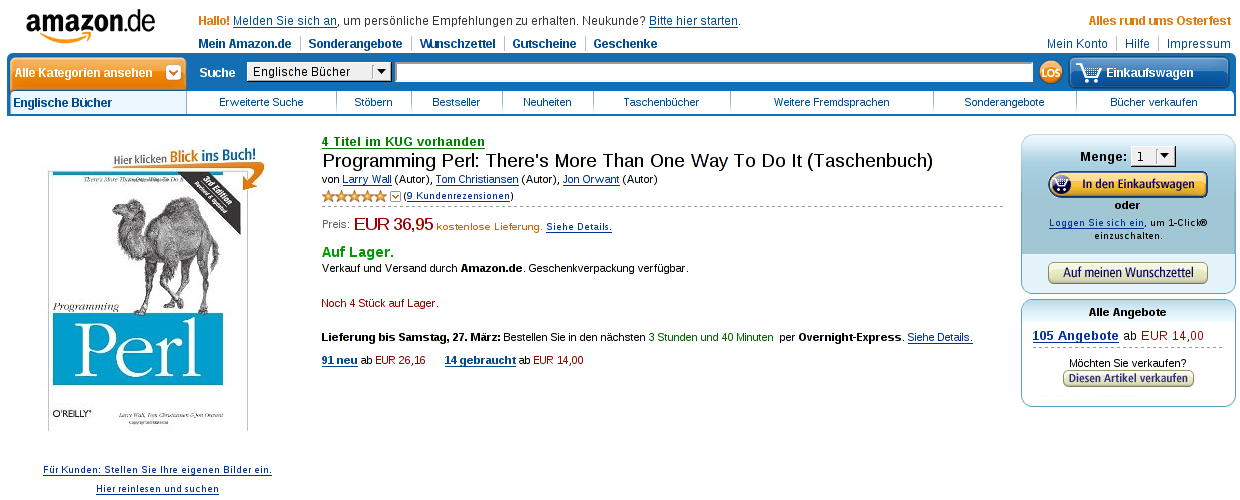
\includegraphics[width=15cm]{bib20-kug-mashups_bilder/greasemonkey_amazon.png}
    \end{minipage}
    \caption{KUG-Bestand in Amazon: Katalognachweise dort anzeigen, wo der Nutzer ist}
  \label{bild:amazon}
\end{figure}

Dieser Konnektor wird verwendet, um dem Endnutzer über die
Firefox-Erweiterung GreaseMonkey in seinen Recherchen bei Amazon oder
Google Bücher direkt die Verfügbarkeit des jeweiligen Titel im KUG
anzuzeigen. Falls der Titel selbst nicht vorhanden ist, werden
stattdessen die Nachweise der anderen Auflagen usw. ausgegeben. Auf
diese Weise können die Nachweise lokaler Bestände dort angezeigt
werden, wo sich der Nutzer befindet (Abbildung \ref{bild:amazon}).
  
Auch bei unseren Lieferanten wird dieser Konnektor im Rahmen der
Vorakzession in Approval-Plänen genutzt, um die Verfügbarkeit eines
Titels nicht mehr händisch am USB-OPAC durch\-führen zu müssen, sondern
automatisch über diesen Web-Service.

Für die Auslieferung maschinenlesbarer bibliographischer Informationen
zu einzelnen Titeln verwendet der KUG die
unAPI-Schnittstelle\cite{Chudnov:2006}. Über diese können die
Titelinformationen "= anders als bei COinS\footnote{OpenURL COinS: A
  Convention to Embed Bibliographic Metadata in HTML
  \path|http://ocoins.info/| . Zuletzt besucht am: 26.3.2010} "= in
verschiedenen Formaten ausgegeben werden, wie z.B. BibTeX, MODS, DC
"= oder METS, wie im Fall von WikiSource.

Der KUG hat die bibliographischen Nachweise von Digitalisaten in
WikiSource zusammen mit der Struktur der Digitalisate in einem eigenen
Katalog abgelegt. Diese Strukturinformationen sind über unAPI im
METS-Format abfragbar und können damit direkt an den
DFG-Viewer\footnote{\path|http://dfg-viewer.de/| Zuletzt besucht am:
  26.3.2010} zur Anzeige des Digitalisats übergeben werden. Durch die
Kombination offener Daten von WikiSource, einem Mashup-fähigen Dienst
der USB und einem der DFG konnte so für unsere Nutzer ein Mehrwert
geschaffen werden, der das Potential von Mashups sehr klar
verdeutlicht.

Aber auch andere Programme nutzen direkt die unAPI-Schnittstelle. Ein
sehr prominentes Beispiel ist Zotero, ebenfalls eine Erweiterung des
Web-Browsers Firefox. Mit Zotero kann der Nutzer via unAPI direkt aus
der Einzeltrefferanzeige deren bibliographische Daten übernehmen.

Dies waren nur einige Beispiele, die aber zeigen, dass es nicht nur
sinnvoll ist Mashups selbst zu nutzen, sondern dass es mindestens
ebenso wichtig ist, sein eigenes System so anzupassen, damit dieses
durch offene Schnittstellen auch selbst über Mashups eingebunden
werden kann.

\section{Allgemeine Vernetzungen zwischen Titeln}

Bisher wurden bereits einige Beispiele für das Prinzip Serendipity
"`Sinnvolles finden, das gar nicht gesucht wurde"' angesprochen. Die
Erweiterung des Kataloges um zusätzliche thematische Querverbindungen
zwischen verschiedenen Titeln ist daher eine für den Endnutzer sehr
wesentliche Eigenschaft einer Rechercheanwendung.

Daher versuchen wir im KUG fortlaufend aus den vorhandenen Daten
möglichst automatisch weiterführende Informationen und Vernetzungen
zwischen Titeln zu identifizieren und dann einer sinnvollen Nutzung
zuzuführen.

Die allgemeinen bibliographischen Informationen eines Titels sind hier
bereits ein guter Ansatzpunkt. Querverbindungen über Personen,
Körperschaften, Schlagworte und Systematiken haben sich bereits seit
vielen Jahren durchgesetzt.

Man kann sich nun aber auch weitere Fragen stellen, um thematisch
potentiell benachbarte Titel aufzuspüren. Haben die verschiedenen
Verfasser des aktuellen Titels beispielsweise mit weiteren Personen in
anderen Titeln zusammengearbeitet? Gibt es hier eventuell Häufungen?
Diese könnten dem Recherchierenden sicherlich hilfreich sein. Oder,
welche anderen Schlagworte kommen bei anderen Titeln zusammen mit den
Schlagworten des aktuellen Titels vor? Wie sieht es hier mit Häufungen
aus?

Derartige Informationen werden im KUG beim Aufruf eines Titels
augenblicklich bestimmt und dem Nutzer als weitere
"`Entdeckungsmöglichkeit"' über Wortwolken angeboten.

Ebenso lassen sich auch Literaturlisten auswerten, die von Nutzern
eingegeben und öffentlich freigegeben wurden. Welche anderen
Literaturlisten hat der Nutzer sonst noch erstellt? Könnte da
vielleicht etwas Interessantes dabei sein? Kommen Titel der aktuellen
Literaturliste vielleicht in anderen Literaturlisten vor? Könnte ich
vielleicht hier auf neue Titel stoßen, an die ich bisher noch gar
nicht gedacht habe? Auch diese beiden Vernetzungen für Literaturlisten
werden im KUG umgesetzt.

Andere Vernetzungen lassen sich aus Nutzungsanalysen bestimmen. Dazu
bietet die KUG-Plattform eine allgemeine Statistikdatenbank an, in der
beliebige nutzungsbedingte Ereignisse abgelegt und später ausgewertet
werden können. Nur so erhält die USB Köln als Systembetreiber u.a.
diejenigen Informationen, anhand derer sie den Dienst verbessern kann.

Eine sehr wesentliche Information, die aus einer Analyse der
KUG-Nutzung gewonnen werden kann, sind Literaturempfehlungen. Die
Empfehlungen werden anhand eines speziellen Algorithmus auf Grundlage
aufgerufener Vollanzeigen der Titel bestimmt. Um auch hier einen
maximalen Nutzen für möglichst viele Kataloge zu erzielen, werden
diese Informationen wiederum der zentralen Kataloganreicherung
zugeführt.

\section{Weitere Dienstleistungen aus den Daten der KUG-Plattform}

Außerhalb der Universität zu Köln ist der KUG nahezu ausschließlich
als Recherche-Plattform bekannt. Einige Bibliotheken nutzen unsere
SeeAlso-Dienste, vielfach unbekannt sind jedoch andere
Dienstleistungen, die wir anhand der in der KUG-Plattform gesammelten
Daten lokal an der Universität erbringen.

Wesentlich ist auch hier die lokale Haltung der bibliographischen
Informationen in relationalen Datenbanken. Diese Informationen sind so
abgelegt, dass sie sich "= anders als in vielen Erfassungssystemen "=
bis auf die Kategorieebene ansprechen lassen.

Allein mit Hilfe dieser Informationen können wir bereits für unsere
Bibliotheken als Dienstleistung einen Abgleich zwischen beliebigen
Katalogbeständen anbieten. Diese Aufstellung gemeinsamer Titel in den
jeweiligen Bibliotheken wird in Form einer CSV-Datei geliefert und ist
ein sehr hilfreiches Entscheidungsinstrument für Aussonderungen oder
Zusammenlegungen von Bibliotheken.

\subsection{Beispiel: Bibliotheksführer als E-Book}

Zusätzlich werden in der KUG-Plattform aber nicht nur Katalogdaten
abgelegt, sondern auch Informationen über die zugehörigen
Bibliotheken. Diese Bibliotheksinformationen werden an der USB Köln in
Form eines offiziellen Bibliotheksführers, ehemals in einer aufwändig
hergestellten Print-Version, heute online auf den Webseiten geführt.
Dabei werden u.a. Adressen, Öffnungszeiten, EDV-Ausstattung,
Ansprechpartner, Geo-Koodinaten, Gesamtbestand und vieles mehr
erfasst.

Um diese Informationen vollintegriert in der  KUG-Anwendung
darstellen zu können, werden sie automatisiert aus den Webseiten
extrahiert und kategorisiert in den KUG eingespielt.

\begin{figure}[ht]
    \centering \begin{minipage}[b]{1.0\textwidth}
      \centering 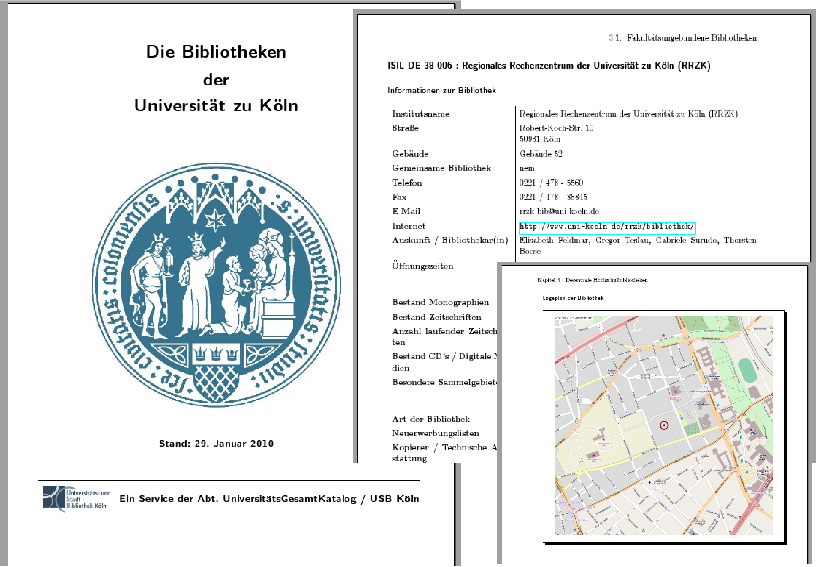
\includegraphics[width=15cm]{bib20-kug-mashups_bilder/bibfuehrer.png}
    \end{minipage}
    \caption{Automatisch aus dem KUG erzeugter Bibliotheksführer als E-Book}
  \label{bild:bibfuehrer}
\end{figure}
 
Es besteht jedoch weiterhin ein großer Bedarf nach einer umfassenden
Gesamtübersicht aller Bibliotheken in einer ausdruckbaren Publikation.
Mit dem KUG als Datenzentrale, in der alle relevanten Informationen
vorliegen, kann die USB Köln einen
Bibliotheksführer\footnote{\path|http://kug.ub.uni-koeln.de/bibliotheksfuehrer/|.
  Zuletzt besucht am: 26.3.2010} im pdf-Format automatisch als weitere
Dienstleistung erzeugen. Da die Erzeugung mit keinem Aufwand verbunden
ist, wird der ausdruckbare Bibliotheksführer täglich erzeugt und ist
entsprechend aktuell. Auch in diesem Prozess finden wieder
Mashup-Techniken Anwendung. Anhand der erfassten Geo-Koordinaten einer
jeden Bibliothek wird per Mashup mit dem OpenStreetMap
Projekt\footnote{\path|http://www.openstreetmap.org/|. Zuletzt besucht
  am: 26.3.2010} automatisch ein Lageplan der Bibliothek eingebunden
(Abbildung \ref{bild:bibfuehrer}).

Da im KUG neben den allgemeinen Informationen über die Bibliotheken
gleichzeitig katalog\-spezifische Informationen verfügbar sind, können
aus der Kombination neue Inhalte erzeugt werden. Für den Nutzer
wesentlich ist z.B., wieviele Titel des Gesamtbestandes überhaupt
elektronisch erfasst und damit recherchierbar sind.

Pro Gruppe an Katalogen "= typischerweise fakultätsweise "= werden
daher die von den Bibliotheken gemeldeten Bestandszahlen zusammen mit
der Zahl tatsächlich elektronisch erfasster Titel ausgegeben.
Wünschenswert für den Recherchierenden wären diese Angaben über den
Erfassungsgrad sicherlich auch bezogen auf jede einzelne Bibliothek.
Denn das Hintergrundwissen "`Wie sinnvoll ist es eigentlich, im
Online-Katalog zu suchen? Oder ist es vielleicht doch besser, den
Kartenkatalog zu konsultieren?"' ist entscheidend dafür, dass der
Recherchierende auch zum gesuchten Medium kommt.

Die damit verbundene Problematik geht jedoch weit über die einfache
technische Realisierbarkeit hinaus.

\subsection{Beispiel: Liste der Zeitschriften in der ZDB}

An der USB Köln werden zentral die Nachweise der
Institutszeitschriften in der ZDB geführt. Als Arbeitsinstrument
generieren wir aus dem KUG daher für jedes Institut Listen der
Zeitschriften, die aktuell in der ZDB für dieses Institut gemeldet
sind. Die Institute können anhand dieser Listen dann überprüfen, ob
sich inzwischen Änderungen ergeben haben und uns dies zur Korrektur
der Daten in der ZDB zurückmelden.

Als weiteres Angebot an die Institute werden in diesen Listen zur
Erwerbungs- und Bestandkoordination automatisch auch zusätzlich
Informationen über Parallel-Bestände in anderen Instituten vermerkt.
Als allgemeine Information wird am Anfang der Liste neben der
Gesamtzahl der Zeitschriften im jeweiligen Institut auch die Zahl der
Zeitschriften ausgegeben, die auch in anderen Bibliotheken vorhanden
sind. Bei jeder aufgeführten Zeitschrift werden dann konkret diese
anderen Bibliotheken anhand ihrer Sigel genannt.
   
Diese drei Beispiele zeigen, dass sich aus einer zentralen
Recherche-Plattform in einem Katalogverbund vielfältige
Dienstleistungen für verschiedene Zielgruppen entwickeln lassen, die
über die eigentliche Recherche hinausgehen können.

\section{Neue Möglichkeiten mit offenen Daten}

Schon seit einiger Zeit wird im Bibliothekswesen laut über die
Freigabe der bibliographischen Daten als (Linked) Open Data
nachgedacht "= u.a. in größerem Rahmen bei der Tagung "`Semantik Web
in Bibliotheken"' SWIB09\footnote{Folien und Videos der Vorträge auf
  der Tagungsseite \path|http://www.swib09.de/|. Zuletzt besucht am:
  26.3.2010} im Kontext des Semantic Web.

Kein anderer als der "`Erfinder"' des Web, Tim Berners-Lee,
propagierte\footnote{Berners-Lee, Tim: The year open data went
  worldwide \path|http://www.ted.com/talks/view/id/788| . Zuletzt
  besucht am: 26.3.2010} schon vor einigen Jahren die Freigabe von
Daten, zunächst als Roh-Daten, dann beschrieben durch Web-Standards,
um sie zum integralen Teil des Webs\footnote{Dodds, Leigh: Web
  integrated data
  \path|http://www.slideshare.net/ldodds/web-integrated-data| .
  Zuletzt besucht am: 26.3.2010} zu machen. Diese Daten "= oder Teile
davon "= können dann vielfältig genutzt und kombiniert werden "= in
Anwendungsgebieten, an die man selbst mit seinen Daten eventuell noch
gar nicht gedacht hat.

Auch wir in der USB Köln sehen das immense Potential, das sich mit
vollständig (gemein)freien bibliographischen Daten erreichen lässt. Um
dieses Potential auszuschöpfen, hat die USB Köln zusammen mit
verschiedenen anderen Kölner Bibliotheken und dem
Landesbibliothekszentrum Rheinland-Pfalz (LBZ) in Kooperation mit dem
Hochschulbibliothekszentrum des Landes Nordrhein-Westfalen (hbz) ihre
bibliographischen Daten vollständig für die Allgemeinheit geöffnet "=
in dieser Dimension ein Novum in der deutschen Bibliotheksgeschichte.
Allein die USB gab mehr als 3 Millionen Titelsätze frei, zusammen mit
den anderen Bibliotheken waren es mehr als 5 Millionen. Wenn weitere
Bibliotheken folgen, ließe sich der gemeinsamen Nutzen, den alle aus
den Daten ziehen können, noch weiter erhöhen.

Gerade die bereits vorgestellten und in der KUG-Plattform umgesetzten
Strategien lassen sich durch Open Bibliographic Data deutlich
erweitern und verbessern.

Der Weg hin zu Open Bibliographic Data hat verschiedene
Dimensionen\footnote{Pohl, Adrian: Dimensionen von Open Bibliographic
  Data\newline
  \path|http://www.uebertext.org/2010/03/dimensionen-von-open-bibliographic-data.html|
  . Zuletzt besucht am: 26.3.2010}. Für den konkreten Einsatz sind,
neben der Kostenersparnis durch eine komplette Übernahme von Titeln,
vor allem zwei Bereiche wesentlich: Als Quelle für Anreicherungen mit
externen Inhalten und zur Verankerung des Bibliotheksbestandes im
Netz.

Viele Inhalte aus externen Katalogaufnahmen können zu einer
qualitativen Verbesserung der eigenen Daten beitragen. Dazu gehören
u.a. Schlagworte, Systematikinformationen wie Basisklassifikation (im
GBV und der USB), RVK (im BVB) oder DDC, PND-Nummern, Links zu
digitalisierten Inhaltsverzeichnissen mit OCR-Volltexten,
katalogisierte freie E-Books und vieles mehr. Mit diesen zusätzlichen
Informationen lässt sich "= durch zentrale Anreicherung im KUG oder
expliziten Import in die einzelnen Kataloge "= für den
Recherchierenden der Katalogbestand tiefer thematisch erschließen und
ein deutlich verbesserter Recherche-Dienst anbieten.

Bibliothekskataloge oder -portale sind nicht mehr die ersten
Anlaufstellen, wenn Nutzer heutzutage Informationen zu einem Thema
suchen. Schon 2005 ging aus der Studie "`Perception of Library and
Information Resources"'\footnote{Frage 520: Where electronic
  information searches begin
  \path|http://www.oclc.org/reports/pdfs/Percept\_all.pdf|. Zuletzt
  besucht am: 26.3.2010} von OCLC deutlich hervor, dass für 84 Prozent
der Recherchierenden Suchmaschinen wie Google die erste Wahl sind.
Lediglich 1 Prozent von ihnen beginnen ihre Suche in
Online-Datenbanken oder den Webseiten einer Bibliothek.

Um die Nutzer dort abzuholen, wo sie suchen, müssen die
bibliographischen Daten mit ihren Bestandsinformationen integraler
Teil des Netzes werden. Der einfachste und kostengünstigste Weg ist
die Beschreibung dieser Daten in der Sprache des Web mit RDF durch
geeigneten Ontologien und Veröffentlichung als Open Bibliographic
Data, so dass sie durch Suchmaschinen eingesammelt "= und sinnvoll
verarbeitet werden können. Auch im lokalen Kontext können sich so
Resourcen-orientierte Infrastrukturen\cite{Spinellis:2009} bilden, die
in der Verarbeitung der Informationen neue Perspektiven eröffnen.

Zusätzlich können Querverweise zu anderen Datenquellen, wie z.B. der
Dbpedia\footnote{\path|http://dbpedia.org/About|. Zuletzt besucht am:
  26.3.2010}, LCSH\footnote{Library of Congress Subject Headings
  \path|http://id.loc.gov/authorities/search/|. Zuletzt besucht am:
  26.3.2010} oder STW\footnote{Standard Thesaurus Wirtschaft
  \path|http://www.w3.org/2001/sw/sweo/public/UseCases/ZBW/| Zuletzt
  besucht am: 26.3.2010}, eingebracht werden und so die Daten als
Linked Open Data\footnote{Davis, Ian ; Heath, Tom: The thirty minute
  guide to RDF and Linked Data.
  \newline\path|http://www.slideshare.net/iandavis/30-minute-guide-to-rdf-and-linked-data|
  Zuletzt besucht am: 26.3.2010}{ }\footnote{OPENLINK Software: Deploying
  Linked Data.\newline
  \path|http://virtuoso.openlinksw.com/Whitepapers/html/vdld\_html/VirtDeployingLinkedDataGuide.html|
  Zuletzt besucht am: 26.3.2010} in einem semantischen Web noch
wertvoller machen.  Durch geeignete Abfragesysteme und Sprachen wie
SPARQL lassen sich im Semantic Web durch die Querverbindungen zwischen
vielen verschiedenen Datenquellen Fragestellungen beantworten, die so
bisher nicht effizient möglich waren, wie in einem Beispiel von Juan
Sequeda: "`Football Players who went to the University of Texas at
Austin, played for the Dallas Cowboys as
Cornerback"'.\footnote{Sequeda, Juan: Introduction to Linked Data.
  International Semantic Web Conference. 2009
  \path|http://www.slideshare.net/juansequeda/introduction-to-linked-data-2341398|
  Zuletzt besucht am: 26.3.2010}

\section{Zusammenfassung}

Anhand der KUG-Plattform an der USB Köln wurden verschiedene Beispiele
dargestellt, wie durch die besondere Herausforderung vieler,
heterogener Kataloge andere Wege beschritten werden mussten als bei
einem einzelnen Katalog. Die dabei umgesetzten Lösungen und Prinzipien
"= Anreicherungen, Mashups und Vernetzungen "= sind jedoch so
allgemein, dass sie sich auf eine Vielzahl an Arten von Katalogen "=
einzelne, getrennte oder verteilte "= anwenden lassen. Erst durch
ihren Einsatz kann für den Recherchierenden im Umfeld heterogener
Kataloge ein Höchstmaß an Homogenität erreicht werden.

Speziell die zentrale Anreicherungsdatenbank ist dabei ein zentrales
Bindeglied zwischen den ansonsten einzelnen Katalogbeständen im KUG.
Sie bietet sich mit den dort enthaltenen Informationen als
"`Andockpunkt"' für externe Mashups mit dem KUG an, z.B. über den
SeeAlso-Konnektor.

Zentral bei der Realisierung und Weiterentwicklung der KUG-Plattform
war die Loslösung des Blicks von einem einzelnen Katalog "`im Vakuum"'
und die Ausweitung auf einen größeren Kontext: Der einzelne Katalog im
Verbund mit anderen Katalogen, der Katalogverbund als Teil des Netzes
mit vielen Katalogen und Verbünden. Dadurch wurden fast automatisch
allgemeine Techniken des Web 2.0 adaptiert, die sich in einem zutiefst
heterogenen und schnell wandelnden globalen Netz "= dem Internet "= in
ihrer praktischen Anwendbarkeit durchgesetzt haben.

Niemand kann vorhersagen, welche Dienste oder Daten als nächstes
sinnvoll in eine bibliothekarische Rechercheanwendung eingebunden
werden können. Auch die Anforderungen an eigene Schnittstellen, über
die man zwischen Bibliotheken und Verbünden neue Dienste gemeinsam
erschaffen kann, entwickeln sich ständig weiter.

Um mit seinem eigenen Recherchedienst in dieser Zeit des fortwährenden
Wandels überhaupt "`manövrierfähig"' zu sein, ist die Flexibilität,
geeignete Erweiterungen mit möglichst geringem Aufwand selbst
vornehmen zu können, so außerordentlich elementar. Dazu bedarf es
Systeme, die eine eben solche Flexibilität ermöglichen und die dabei
so effizient sind, dass sie den notwendigen Aufwand für Anpassungen,
Erweiterungen und Betrieb minimieren.

Der KUG und andere eigenentwickelte Systeme, wie
vuFind\footnote{\path|http://vufind.org/| Zuletzt besucht am:
  26.3.2010},
Heidi\footnote{\path|http://www.ub.uni-heidelberg.de/helios/kataloge/heidi.html|
  Zuletzt besucht am: 26.3.2010},
beluga\footnote{\path|http://beluga.sub.uni-hamburg.de/| Zuletzt
  besucht am: 26.3.2010} oder
XOPAC\footnote{\path|http://www.xopac.org/| Zuletzt besucht am:
  26.3.2010}, sind gute Beispiele dafür, den Betreuungsaufwand für
eine schwerfällige, proprietäre Lösung sinnvoller in die
(Weiter-)Entwicklung und Anpassung bestehender Open Source-Sys\-te\-me zu
investieren.

Dazu kommen weitere Vorteile, denn gerade die beiden damit
zusammenhängenden Faktoren "= die Auseinandersetzung mit aktuellen und
zukünftigen Themen sowie die anschließende selbständige Umsetzung im
Rahmen eines vollständig offenen Systems "= sind wesentlich für den
Aufbau von Wissen und Kompetenz in Bibliotheken\footnote{Vgl. Analyse
  von Christensen, Anne ; Christof, Jürgen: beluga "= Die Hamburger
  Rechercheplattform zur Literaturversorgung virtueller Lernräume.
  2007.\newline
  \path|http://beluga.sub.uni-hamburg.de/blog/wp-content/uploads/2007/10/jourfixe\_2007.pdf|
  Zuletzt besucht am: 26.3.2010}.

Während bei einem proprietären System oft nur produktspezifisches
Spartenwissen aufgebaut wird, geschieht der Wissensaufbau bei
aktuellen, vollständig offenen Systemen in verbreiteten
Basistechniken, die sich auch in anderen Projekten sehr gut anwenden
lassen und so erst einen wirtschaftlichen und nachhaltigen Betrieb mit
begrenzten Finanzmitteln und Personal - für den Nutzer -
gewährleisten.

\newpage

\begin{thebibliography}{ChBr82}
\originalTeX

\bibitem[Bauer 2004]{Bauer:2004} Bauer, Delia: \emph{Vom zweischichtigen
    Bibliothekssystem zur funktionalen Einschichtigkeit: Problematik
    eines Strukturkonzepts am Beispiel der Universitäts- und
    Stadtbibliothek Köln.} Band 43. 2004. Kölner Arbeitspapiere zur
  Bibliotheks- und Informationswissenschaft.\newline
  \path|http://www.fbi.fh-koeln.de/institut/papers/kabi/band.php?key=54|\newline
  Zuletzt besucht am: 26.3.2010

\bibitem[Chudnow et al 2006]{Chudnov:2006} Daniel~Chudnov~et~al: \emph{Introducing
    unAPI}, in: Ariadne. Issue 48 (July 2006)\newline
  \path|http://www.ariadne.ac.uk/issue48/chudnov-et-al/|\newline Zuletzt
  besucht am: 26.3.2010

\bibitem[Flimm 2007]{Flimm:2007} Flimm, Oliver: \emph{Die Open-Source-Software OpenBib an der USB Köln : Überblick und Entwicklungen in Richtung OPAC 2.0.} in: BIBLIOTHEK. Forschung und Praxis, Jg. 31 (2007) Nr. 2. \path|http://eprints.rclis.org/9891/|\newline Zuletzt besucht am: 26.3.2010

\bibitem[Hahn Schulze 2009]{Hahn:2009} Hahn, Ulrich ; Schulze,
  Matthias: \emph{Katalogerweiterungen, Mashups  und Elemente der "`Bibliothek 2.0"' in der Praxis.} in: Bibliotheksdienst 43. Jg. (2009), H. 1, S. 20-38 \newline\path|http://www.zlb.de/aktivitaeten/bd_neu/heftinhalte2009/Erschliessung010109.pdf|\newline Zuletzt besucht am: 26.3.2010

\bibitem[Spinellis et al 2009]{Spinellis:2009} Spinellis et al:
  \emph{Resource-Oriented Architectures : Being "`In the
    Web"'}. O'Reilly. 2009. In: Beautiful Architecture - ISBN
    978-0-596-51798-4

\bibitem[Stelzenmüller 2008]{Stelzenmueller:2008} Stelzenmüller,
  Christian: \emph{Mashups in Bibliotheken. Untersuchung der
    Verbreitung von Mashups auf Webseiten wissenschaftlicher
    Bibliotheken und Erstellung eines praktischen
    Beispiels}. Stuttgart. 2008\newline
  \path|http://opus.bsz-bw.de/hdms/volltexte/2008/654/|\newline Zuletzt
  besucht am: 26.3.2010

\bibitem[Tonkin et al 2008]{Tonkin:2008} Tonkin et al:
  \emph{Collaborative and social tagging networks}. in: Ariadne. Issue
  54 (January 2008)\newline
  \path|http://www.ariadne.ac.uk/issue54/tonkin-et-al/|\newline Zuletzt
  besucht am: 26.3.2010

\bibitem[Voß 2007]{Voss:2007} Voß, Jakob: \emph{Tagging, Folksometries
    and Co - Renaissance of Manual Indexing?}.  Proceedings of the
    International Symposium of Information
    Science. \newline\path|http://arxiv.org/abs/cs/0701072|\newline Zuletzt besucht
    am: 26.3.2010

\bibitem[Voß 2008]{Voss:2008} Voß, Jakob: \emph{SeeAlso : A Simple
    Linkserver Protocol}. in: Ariadne, Issue 57 (October 2008)\newline
  \path|http://www.ariadne.ac.uk/issue57/voss|\newline Zuletzt besucht am:
  26.3.2010

\end{thebibliography}
\germanTeX

\newpage
\fancyhead[L]{}
%\thispagestyle{empty}
\section*{Kurz-Biographie des Autors}
Oliver Flimm, Jahrgang 1969, ist Diplom-Physiker und als Administrator
sowie Programmierer im Bereich Unix/Linux seit 1991 tätig. Während
seines Studiums der Physik mit Nebenfach Informatik arbeitete er an
der USB Köln und betreute dort technisch das Projekt
InstitutsGesamtKatalog (IGK). Nach Abschluss seines Studiums übernahm
er dort als wissenschaftlicher Mitarbeiter neben seiner Tätigkeit im
Bereich Unix/Linux-Administration und -Programmierung u.a. die
technische Durchführung verschiedener Projekte -- insbesondere des
KUG-Projektes.

\section*{Anschrift des Autors}

Oliver Flimm\newline
Universitäts- und Stadtbibliothek Köln\newline
Dezernat 1 - EDV\newline
Universitätsstr. 33\newline
D-50931 Köln\newline
E-Mail: flimm@ub.uni-koeln.de\newline


\section*{Lizenz}

Der Artikel steht unter der Creative Commons CC-BY Lizenz.

Er wurde veröffentlicht in:

\emph{Handbuch Bibliothek 2.0}, Hrsg. von Julia Bergman und Patrick
Danowski, Berlin, New York: De Gruyter Saur, September 2010, S. 293-316. - ISBN 978-3-11-023210-3


\end{document}

%%% Local Variables: 
%%% mode: latex
%%% TeX-master: t
%%% End: 
